\documentclass[__main__.tex]{subfiles}
\begin{document}

\qtitle{С}{10}
Работа в электростатическом поле, потенциальность электростатического поля. Потенциальная энергия точечного заряда $q$ в поле, создаваемом системой точечных зарядов $Q_j$.\\

Рассмотрим работу сил в электрическом поле, создаваемом неизменным во времени распределенным зарядом, т.е. электростатическом поле.
\begin{figure}[h]
    \llabel{c101}
    \center{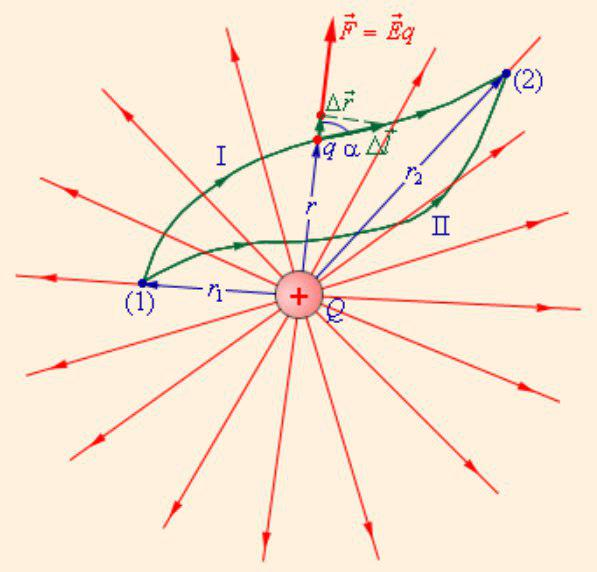
\includegraphics[width=0.5\linewidth]{c-10-1}}
    \caption{Работа кулоновских сил при перемещении заряда $q$ зависит только от расстояний $r_1$ и $r_2$ начальной и конечной точек траектории}
\end{figure}

На рисунке изображены силовые линии кулоновского поля точечного заряда $Q$ и две различные траектории перемещения пробного заряда $q$ из начальной точки (1) в конечную точку (2). На одной из траекторий выделено малое перемещение $\Delta l$. Работа $\Delta A$ кулоновских сил на этом перемещении равна
\begin{gather}
    \llabel{c10-1}
    \Delta A = F\Delta{l}\cos\alpha = Eq\Delta r = \frac{1}{4\pi\varepsilon_0}\frac{Qq}{r^2}\Delta r
\end{gather}
Таким образом, работа на малом перемещении зависит только от расстояния $r$ между зарядами и его изменения $\Delta r$. Если выражение (\lref{c10-1}) проинтегрировать на интервале от $r=r_1$ до $r=r_2$, то можно получить
\begin{gather*}
    A = \int_{r_1}^{r_2}Eqdr = \frac{Qq}{4\pi\varepsilon_0}\left(\frac{1}{r_1}-\frac{1}{r_2}\right)
\end{gather*}
Полученный результат не зависит от формы траектории. На траекториях I и II, изображенных на рисунке, работы кулоновских сил одинаковы. Если на одной из траекторий изменить направление перемещения заряда $q$ на противоположное, то работа изменит знак. Отсюда следует, что на замкнутой траектории работа кулоновских сил равна нулю.\\\\
Если электростатическое поле создается совокупностью точечных зарядов $Q_j$, то при перемещении пробного заряда $q$ работа $A$ результирующего поля в соответствии с принципом суперпозиции будет складываться из работа $A_j$  кулоновских полей точечных зарядов
\begin{gather*}
    A = \sum A_j
\end{gather*}
Т.к каждый член суммы $A_j$ не зависит от формы траектории, то и полная работа $A$ результирующего поля не зависит от пути и определяется только положением начальной и конечной точек.
\begin{definition}
    Поле называется \textbf{потенциальным} если работа сил этого поля при перемещении заряда по любой замкнутой траектории равна нулю.
\end{definition}
Свойство потенциальности электростатического поля позволяет ввести понятие потенциальной энергии заряда в электрическом поле. Для этого в пространстве выбирается некоторая точка $A$, и потенциальная энергия заряда $q$, помещенного в эту точку, принимается равной нулю. Потенциальная энергия заряда $q$, помещенного в любую точку $B$ пространства, относительно фиксированной точки $A$ равна работе $A_{BA}$, которую совершит электростатическое поле при перемещении заряда $q$ из точки $B$ в точку $A$:
\begin{gather*}
    W = A_{BA}
\end{gather*}
В электростатике энергию принято обозначать буквой $W$, так как буквой $E$ обозначают напряженность поля.
\end{document}